\documentclass[12pt]{scrartcl}
\input{../styles/Packages.tex}
\input{../styles/FormatAndHeader.tex}
\usepackage{graphicx}

\setcounter{sheetnr}{5} % Nummer des Übungsblattes
\setcounter{exnum}{2} % Nummer der Aufgabe

% Beginn des eigentlichen Dokuments

\begin{document}

% Aufgabe 2
\exercise{Kollisionsabfrage mithilfe einer Gitterstruktur}
  (d) Im Vergleich zu einem Ansatz basierend auf einem uniformen Gitter hat die Verwendung von Quadtrees weniger Speicherplatzbedarf. Aber es braucht mehr Zeit für Suchanfragen.

% Aufgabe 3
\exercise{kD-Baum}
\begin{enumerate}
  \item kD-Baum
  
  \includegraphics[scale=0.8]{kD-Baum.eps}

  \item die Erstellung des kD-Baums\\

    \begin{figure}[!h]
      \centering
      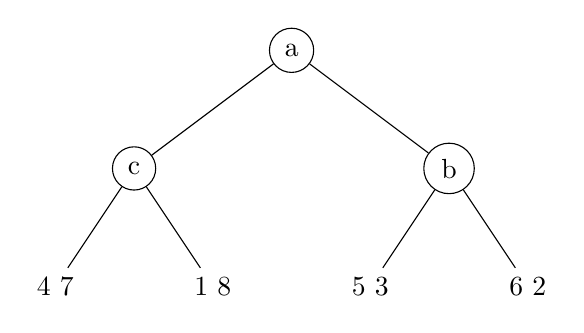
\begin{tikzpicture}
         \node[circle, draw] (a) {a} [level/.style ={sibling distance=40mm/#1}]
          child{node[circle, draw] (b) {c}
            child{node (c) {4 7}}
            child{node (d) {1 8}}
            }
          child{node[circle, draw] (e) {b}
            child{node (f) {5 3}}
            child{node (g) {6 2}}
            };
      \end{tikzpicture}
      \caption{Schnitt 3}
      \label{fig:baum}
      \end{figure}

\newpage\

    \begin{figure}[!h]
      \centering
      \begin{tikzpicture}
         \node[circle, draw] (a) {a} [level/.style ={sibling distance=40mm/#1}]
          child{node[circle, draw] (b) {c}
            child{node (c) {4 7}}
            child{node (d) {1 8}}
            }
          child{node[circle, draw] (e) {b}
            child{node (f) {5 3}}
            child{node[circle, draw] (g) {d}
              child{node (h) {6}}
              child{node (i) {2}}
              }
            };
      \end{tikzpicture}
      \caption{Schnitt 4}
      \label{fig:baum}
      \end{figure}

    \begin{figure}[!h]
      \centering
      \begin{tikzpicture}
         \node[circle, draw] (a) {a} [level/.style ={sibling distance=40mm/#1}]
          child{node[circle, draw] (b) {c}
            child{node (c) {4 7}}
            child{node (d) {1 8}}
            }
          child{node[circle, draw] (e) {b}
            child{node[circle, draw] (f) {e}
              child{node (g) {5}}
              child{node (h) {3}}
              }
            child{node[circle, draw] (i) {d}
              child{node (j) {6}}
              child{node (k) {2}}
              }
            };
      \end{tikzpicture}
      \caption{Schnitt 5}
      \label{fig:baum}
      \end{figure}

    \begin{figure}[!h]
      \centering
      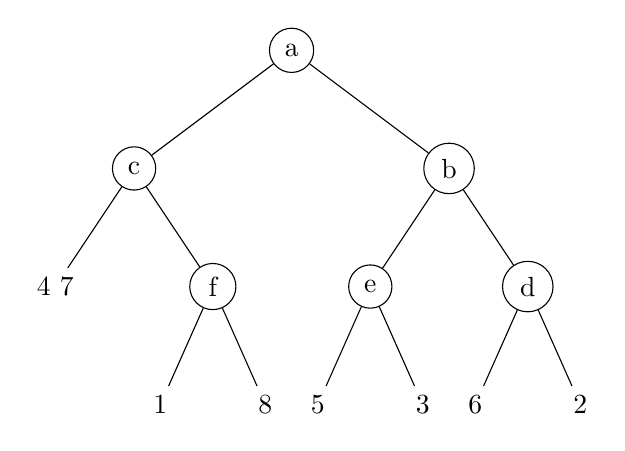
\begin{tikzpicture}
         \node[circle, draw] (a) {a} [level/.style ={sibling distance=40mm/#1}]
          child{node[circle, draw] (b) {c}
            child{node (c) {4 7}}
            child{node[circle, draw] (d) {f}
              child{node (e) {1}}
              child{node (f) {8}}
              }
            }
          child{node[circle, draw] (g) {b}
            child{node[circle, draw] (h) {e}
              child{node (i) {5}}
              child{node (j) {3}}
              }
            child{node[circle, draw] (k) {d}
              child{node (l) {6}}
              child{node (m) {2}}
              }
            };
      \end{tikzpicture}
      \caption{Schnitt 6}
      \label{fig:baum}
      \end{figure}

\newpage\

     \begin{figure}[!h]
      \centering
      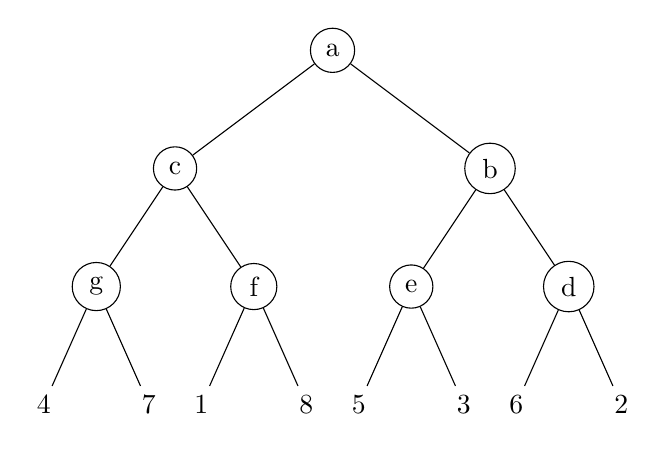
\begin{tikzpicture}
         \node[circle, draw] (a) {a} [level/.style ={sibling distance=40mm/#1}]
          child{node[circle, draw] (b) {c}
            child{node[circle, draw] (c) {g}
               child{node (d) {4}}
              child{node (e) {7}}
              }
            child{node[circle, draw] (f) {f}
              child{node (g) {1}}
              child{node (h) {8}}
              }
            }
          child{node[circle, draw] (i) {b}
            child{node[circle, draw] (j) {e}
              child{node (k) {5}}
              child{node (l) {3}}
              }
            child{node[circle, draw] (m) {d}
              child{node (n) {6}}
              child{node (o) {2}}
              }
            };
      \end{tikzpicture}
      \caption{Schnitt 7}
      \label{fig:baum}
      \end{figure}

  \item Traversierung des Baumes: a->c->f\\
      Für Ebene a, eine Vergleichsoperation.\\
      Für Ebene c, eine Vergleichsoperation.\\
      Für Ebene f, eine Vergleichsoperation.\\

  \item Im worst case: $O(logn)$.\\
          Im best case: $O(logn)$.\\
          Im diesem Fall ist der kD-Baum AVL-Baum. Für die Suchanfragen sind die $O$-Notation für worst case und best case $O(logn)$.\\

  \item Im worst case: $O(n)$.\\
          Im best case: $O(1)$.\\
          Wenn jedes mal eine neue Ebene dazu hinzugefügt wird, liegt auf einer Seite der Ebene nur ein Element, wie z.B.,\\
          \begin{figure}[!h]
          \centering
          \begin{tikzpicture}
          \node[circle, draw] (a) {a} [level/.style ={sibling distance=40mm/#1}]
          child{node (b) {1}}
          child{node[circle, draw] (c) {b}
            child{node (d) {2}}
            child{node[circle, draw] (e) {c}
              child{node (f) {3}}
              child{node[circle, draw] (g) {d}
                child{node (h) {4}}
                child{node (i) {...}}
                }
              }
            };
          \end{tikzpicture}
          \end{figure}

          Für best case, nur 1 Schritt nötig, deshalb $O(1)$.\\
          Für worst case, wenn es $n$ Objekte gibt, wird es insgesamt n Schritte nötig, deshalb $O(n)$.\\
\Delta 
\end{enumerate}

\end{document}
